% !TeX root = ../../main.tex
\chapter{Implementation}
\label{chapter:scafi3-arch-reification}

This chapter discusses the instantiation of the proposed abstract architecture described in \Cref{chapter:contribution} to ScaFi3.
%
\todo{link to de luigi thesis for pure core module, that is not part of this work}

\todo{description of the flow}

\todo{high level architecture modules view}

\todo{project structure - shared, jvm-native, js-native, js, native, jvm and expect/actual Scala mechanism}

\section{High level architecture}

The overview of the ScaFi3 architecture is shown in \Cref{fig:scafi3-architecture}, highlighting the main modules and their relationships.
%
\begin{figure}
    \centering
    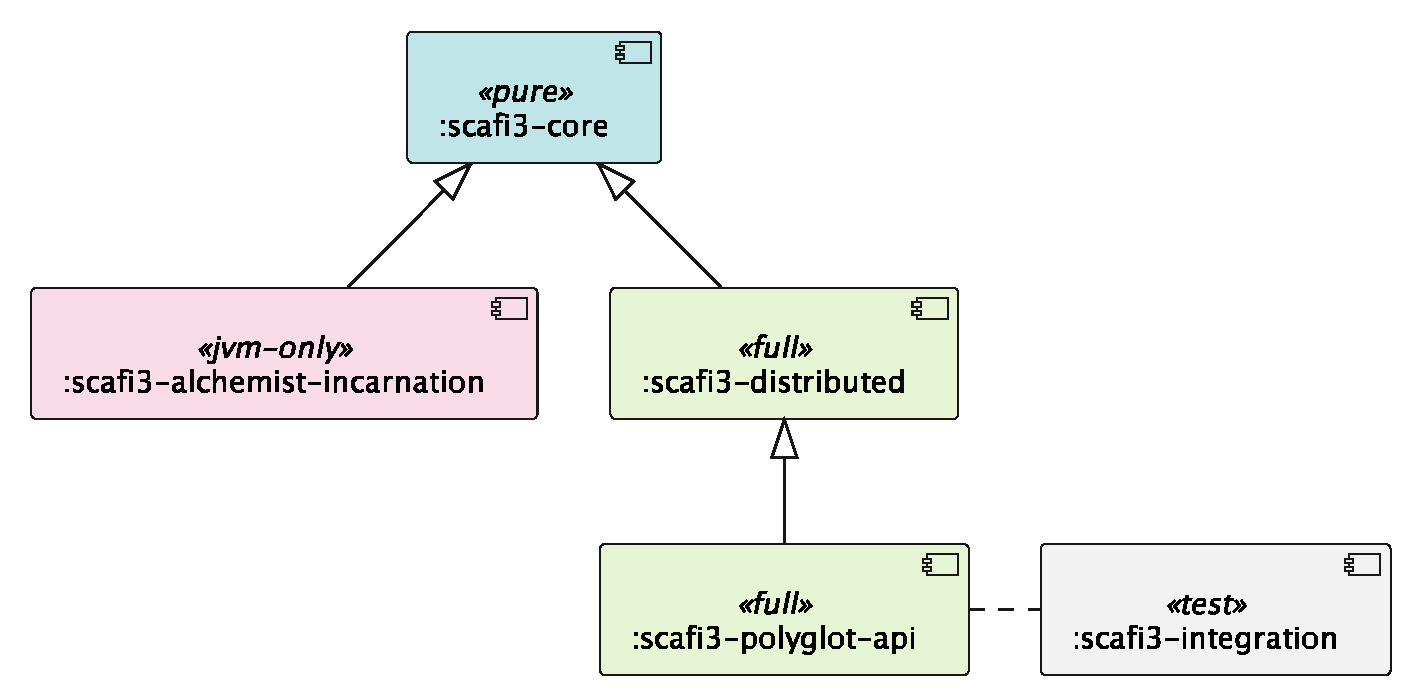
\includegraphics[width=0.7\textwidth]{resources/schemas/scafi3-architecture.eps}
    \caption{UML component diagram of the ScaFi3 architecture.}
    \label{fig:scafi3-architecture}
\end{figure}

\section{Infrastructure module}

\subsection{Distribution module}

Enabling distribution in ScaFi3 requires implementing an abstract network manager that is able to send and receive Value Trees \todo{in context add Value Tree} from and to neighbor devices.
%
The AC framework abstract over the specific protocol used to communicate with neighbors and their discovery mechanism, allowing the implementation of different network managers for different protocols and scenarios.

As an initial step in ScaFi3's evolution toward full-featured distributed capabilities, a socket-based network manager has been implemented. 
%
This foundation layer employs stream, TCP-based connection-oriented sockets, intentionally prioritizing core communication reliability over advanced distributed features, which remain subjects for future work.
%
Indeed, despite the low-level nature of sockets, they provide a foundational abstraction layer that many higher-level protocols ultimately rely upon (such as HTTP, MQTT, etc.), making them a suitable starting point for building extensible communication mechanisms.
%
Consequently, as shown in \Cref{fig:socket-network-manager-architecture}, each device is bound to a specific endpoint (IP address and port) and communicates point-to-point with its neighbors.
%
\begin{figure}
    \centering
    \includegraphics[width=\textwidth]{resources/img/socket-network-manager.pdf}
    \caption{Socket-based network manager high level architecture.}
    \label{fig:socket-network-manager-architecture}
\end{figure}

The UML class diagram of the socket-based network manager is shown in \Cref{fig:socket-network-manager-design}.
%
It adopts an asynchronous design leveraging Scala's Future-based API and comprises two primary active components that operate concurrently to handle bidirectional communication:
%
\begin{itemize}
    \item the incoming connection \texttt{Listener}, continuously listening for incoming messages from neighbor devices. Received messages are stored in a thread-safe \texttt{Map} that retains only the most recent message from each neighbor, according to a configurable \texttt{Retention Policy} that defines, in absence of new messages, how long a message should be retained before being discarded. The up-to-date view of all the received neighbor messages, a.k.a. their Value Trees, is made available to the ScaFi Engine through the \texttt{receive} method at the beginning of each round of computation;
    \item the outgoing message channel, providing a non-blocking interface for message transmission. Upon the end of each round of computation, the ScaFi Engine invokes the \texttt{send} method of the network manager to dispatch the device's current Value Tree to all its neighbors. For each neighbor, the corresponding Value Tree is pushed through the channel and, asynchronously, dispatched to the corresponding destination. To resolve neighbor addresses the socket-based network manager is mixed in with a \texttt{NeighborhoodResolver}, which provides the necessary endpoint resolution capabilities.
\end{itemize}
%
This dual component design ensure that both incoming and outgoing communications proceed without blocking, a pre-condition for targeting JavaScript environments and at the same time maintain system responsiveness.
%
\begin{figure}
    \centering
    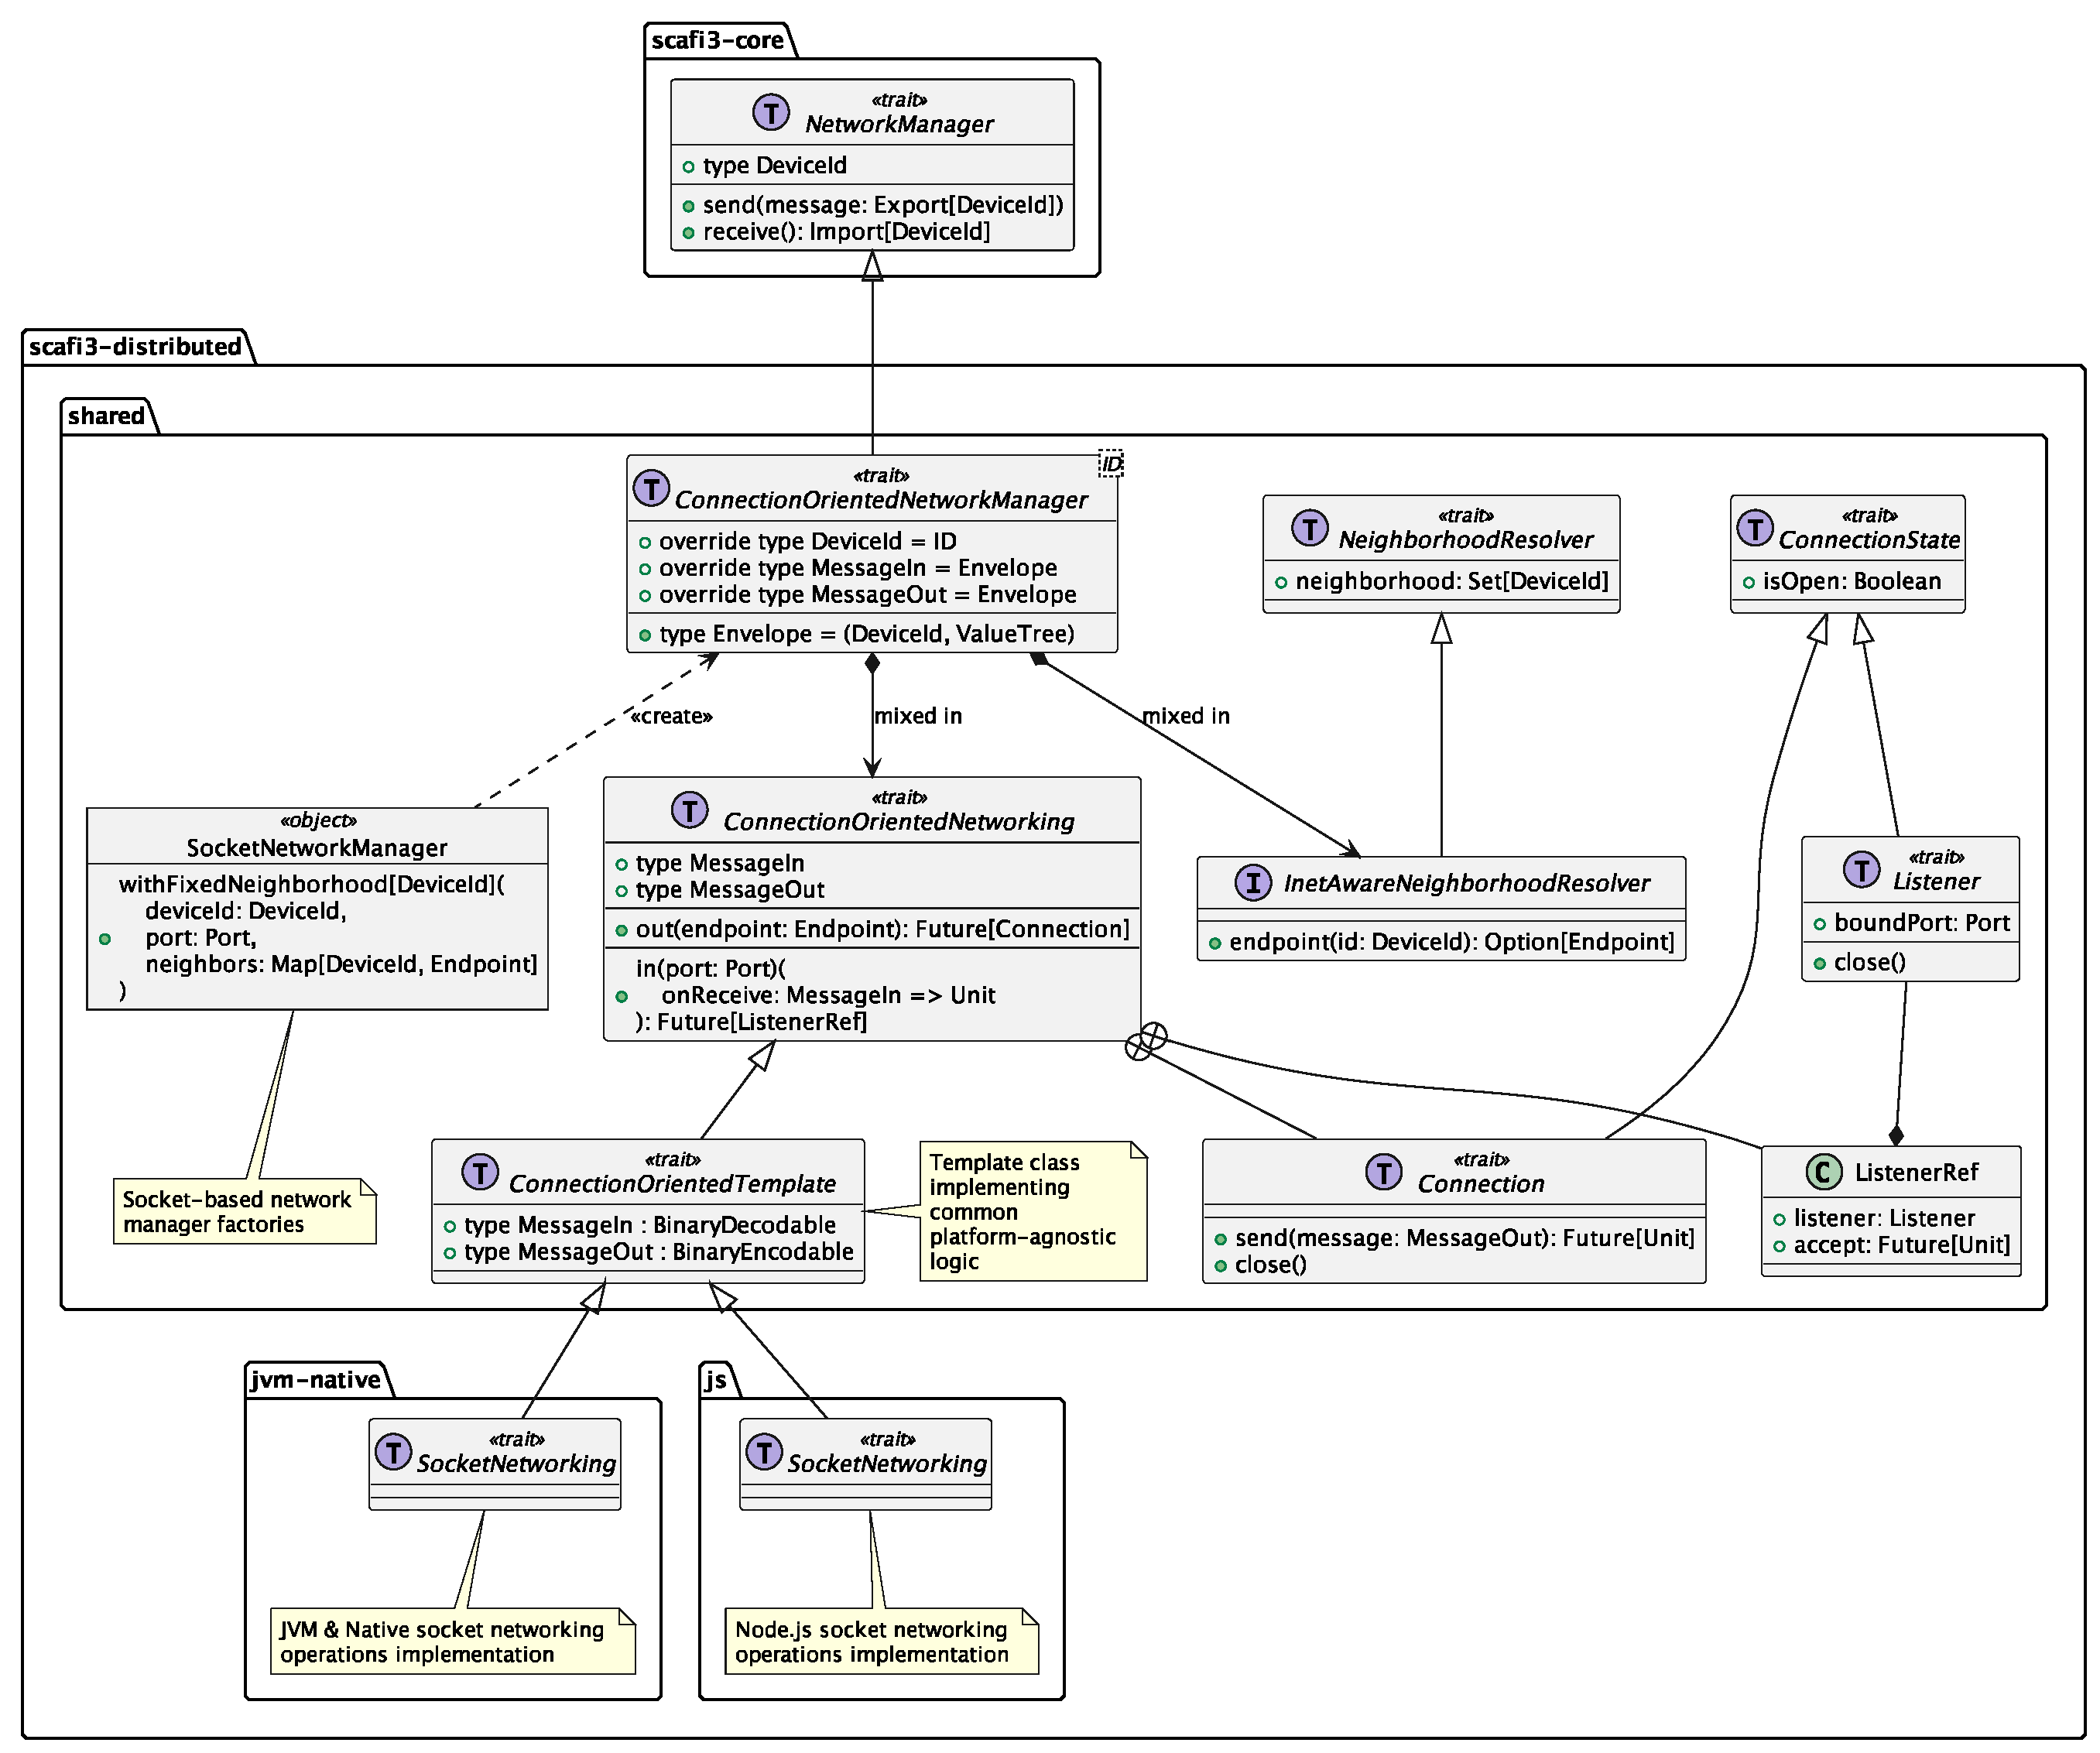
\includegraphics[width=\textwidth]{resources/schemas/socket-distribution.eps}
    \caption{UML diagram of the socket-based network manager design.}
    \label{fig:socket-network-manager-design}
\end{figure}

Remote socket-based communication logic are demanded to the \texttt{ConnectionOrientedNetworking} trait and their platform-specific implementations.
%
Since the absence of a cross-platform socket library supporting both client and server socket programming, two distinct implementations have been provided:
%
\begin{itemize}
    \item one for JVM and Native platforms, leveraging the \texttt{java.net} package available in the standard library. This has been made possible by Scala Native, which have reimplemented the \texttt{java.net} package to provide socket programming capabilities on native platforms. Programmers can thus use the same API on both JVM and Native platforms without any code divergence like they would do in pure Scala JVM applications;
    \item one for JavaScript platforms, leveraging the \texttt{Node.js} library API. For this, the \texttt{net} module of Node.js has been used, through a Scala.js facade that enables calling the Node.js API from Scala.js code. A portion of this facade is shown in \Cref{lst:js-sockets-facade}. This is essentialy the transposition of Node.js API definitions into Scala trait and classes using Scala.js types, annotations and placeholders that, when linked, allow Scala.js code to call the underlying Node.js API.
\end{itemize}

\lstinputlisting[
    language=Scala, 
    label={lst:js-sockets-facade},
    caption={Portion of the Scala.js facade for the Node.js \texttt{net} module.},
    linerange={71-87},
    basicstyle=\ttfamily\scriptsize,
    nolol=true,
]{resources/code/JSSocketsFacade.scala}

Despite targeting all three platforms, the design differs only in platform-specific networking logic, isolated within respective \texttt{SocketNetworking} traits. 
%
This separation leverages Scala's mixin composition and the template method pattern, defining common logic in abstract trait (\texttt{ConnectionOrientedTemplate}) while deferring platform-specific details to specialized mixins.

% \subsection{Protobuf serialization binding}

% \subsection{Platform-specific library abstraction layers}

% \section{Implementation challenges and solutions}
